\documentclass{report}

\usepackage{amsfonts, amsmath, amssymb, amsthm}
\usepackage[margin=1.0in]{geometry}
\usepackage{hyperref}
\usepackage{float}
\usepackage{fancyhdr}
\usepackage{graphicx}
\usepackage{mathrsfs}
\usepackage{comment}

\newcommand{\M}[2]{\mathbb{#1}^{#2}}
\newcommand{\twovector}[2]{\left[ \begin{array}{c} #1 \\ #2 \\ \end{array} \right]}
\newcommand{\threevector}[3]{\left[ \begin{array}{c} #1 \\ #2 \\ #3 \\ \end{array} \right]}
\newcommand{\fourvector}[4]{\left[ \begin{array}{c} #1 \\ #2 \\ #3 \\ #4 \\ \end{array} \right]}
\newcommand{\fivevector}[5]{\left[ \begin{array}{c} #1 \\ #2 \\ #3 \\ #4 \\ #5 \\ \end{array} \right]}
\newcommand{\sixvector}[6]{\left[ \begin{array}{c} #1 \\ #2 \\ #3 \\ #4 \\ #5 \\ #6 \\ \end{array} \right]}
\newcommand{\sevenvector}[7]{\left[ \begin{array}{c} #1 \\ #2 \\ #3 \\ #4 \\ #5 \\ #6 \\ #7 \\ \end{array} \right]}
\newcommand{\eightvector}[8]{\left[ \begin{array}{c} #1 \\ #2 \\ #3 \\ #4 \\ #5 \\ #6 \\ #7 \\ #8 \\ \end{array} \right]}
\newcommand{\ninevector}[9]{\left[ \begin{array}{c} #1 \\ #2 \\ #3 \\ #4 \\ #5 \\ #6 \\ #7 \\ #8 \\ #9 \\ \end{array} \right]}
\newcommand{\nbrack}[1]{\left( #1 \right)}
\newcommand{\bbrack}[1]{\left[ #1 \right]}
\newcommand{\cbrack}[1]{\left\lbrace #1 \right\rbrace}
\newcommand{\abrack}[1]{\left< #1 \right>}
\newcommand{\linebrack}[1]{\left| #1 \right|}
\newcommand{\twomatrix}[4]{\bbrack{
    \begin{array}{cc}
      #1 & #2 \\
      #3 & #4 \\
    \end{array}
  }
}
\newcommand{\threematrix}[9]{\bbrack{
    \begin{array}{ccc}
      #1 & #2 & #3 \\
      #4 & #5 & #6 \\
      #7 & #8 & #9 \\
    \end{array}
  }
}
\newcommand{\Lplc}[1]{\mathscr{L}\bbrack{ #1 } (s)}
\newcommand{\iLplc}[1]{\mathscr{L}^{-1}\bbrack{ #1 } (t)}
\newcommand{\im}{\text{Im}}
\newcommand{\re}{\text{Re}}

\title{Innlevering 7}
\author{Jacob Oliver Bruun}
\date{\today}

\makeatletter
\let\inserttitle\@title
\let\insertauthor\@author
\makeatother

\pagestyle{fancy}
\chead{\insertauthor}
\lhead{\inserttitle}
\rhead{\today}

\parindent 0ex

\begin{document}

\section*{13.1.2}
Plotter
\begin{figure}[H]
  \centering
  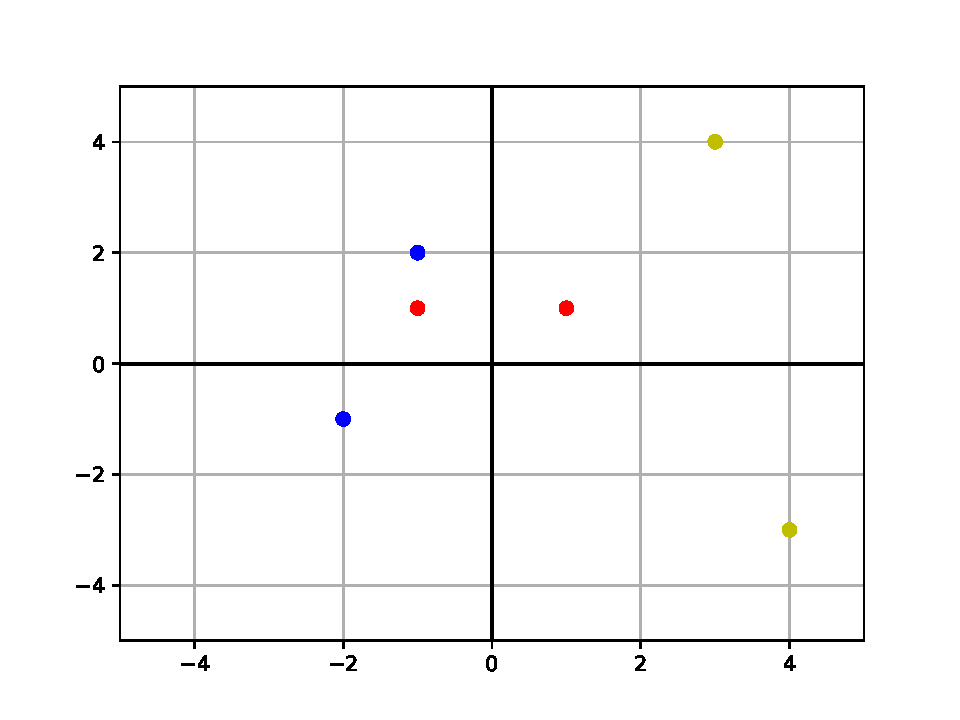
\includegraphics[width=0.6\textwidth]{code/oppg1.pdf}
\end{figure}
og ser da at alle punktene er rotert med $\pi / 2$


\section*{13.1.3}
Ser på
\begin{equation}
  \label{eq:1}
  \frac{x_{1} + iy_{1}}{x_{2} + iy_{2}}
  = \frac{\nbrack{x_{1} + iy_{1}} \nbrack{x_{2} - iy_{2}}}{\nbrack{x_{2} + iy_{2}} \nbrack{x_{2} - iy_{2}}}
  = \frac{ x_{1}x_{2} + y_{1}y_{2} + i \nbrack{ x_{2}y_{1} - x_{1}y_{2} } }{x_{2}^{2}  + y_{2}^{2}}
  = \frac{ x_{1}x_{2} + y_{1}y_{2} }{x_{2}^{2}  + y_{2}^{2}} + i\frac{ x_{2}y_{1} - x_{1}y_{2} }{x_{2}^{2}  + y_{2}^{2}}
\end{equation}
og kan fra dette finne
\begin{equation}
  \label{eq:2}
  \frac{26-18i}{6-2i}
  = \frac{26\cdot 6 + 18\cdot 2}{6^{2} + 2^{2}} + i\frac{-6\cdot 18 + 26\cdot 2}{6^{2} + 2^{2}}
  = \frac{24}{5} - \frac{7}{5}i
\end{equation}


\section*{13.1.14}
Har $z_{1} = -2 + 5i, z_{2} = 3 - i$ og ser på
\begin{equation}
  \label{eq:3}
  \frac{\overline{z_{1}}}{\overline{z_{2}}} = \frac{-2 - 5i}{3 + i} = -\frac{11}{10} - \frac{13}{10}i
\end{equation}
og
\begin{equation}
  \label{eq:4}
  \overline{ \nbrack{ \frac{z_{1}}{z_{2}} } } = \overline{ \nbrack{\frac{-2 + 5i}{3-i}} }
  = \overline{ \nbrack{ -\frac{11}{10} + \frac{13}{10} } } = -\frac{11}{10} - \frac{13}{10}i
\end{equation}


\section*{13.1.16}
Ser på
\begin{equation}
  \label{eq:5}
  \im \frac{1}{z} = \im \frac{1}{x + iy} = -\frac{y}{x^{2} + y^{2}}
\end{equation}
og
\begin{equation}
  \label{eq:6}
  \im \frac{1}{z^{2}} = \im \frac{1}{x^{2} - y^{2} + 2xyi} = \frac{2xy}{x^{4} + y^{4} - 2x^{2}y^{2} + 4x^{2}y^{2}} = \frac{2xy}{x^{4} + y^{4} + 2 x^{2}y^{2}} = \frac{2xy}{\nbrack{ x^{2} + y^{2} }^{2}}
\end{equation}
ved å bruke \eqref{eq:1}.


\section*{13.2.1}
Har generelt
\begin{equation}
  \label{eq:7}
  z = x + iy = \sqrt{x^{2} + y^{2}} e^{i\arctan \frac{y}{x}}
\end{equation}
og kan dermed finne
\begin{equation}
  \label{eq:8}
  1 + i = \sqrt{2} e^{i\frac{\pi}{4}}
\end{equation}


\section*{13.2.8}
Finner først ved \eqref{eq:1}
\begin{equation}
  \label{eq:10}
  \frac{7+4i}{3-2i} = 1 + 2i
\end{equation}
bruker så \eqref{eq:7} og finner
\begin{equation}
  \label{eq:9}
  1 + 2i = \sqrt{5} e^{i\arctan 2}
\end{equation}


\section*{13.2.11}
Ser på
\begin{equation}
  \label{eq:11}
  \arg \nbrack{\sqrt{3} \pm i} = \arctan \pm\frac{1}{\sqrt{3}} = \pm \frac{\pi}{6}
\end{equation}



\section*{13.2.21}
Skal finne $z$ slik at
\begin{equation}
  \label{eq:12}
  z^{3} = r^{3} e^{3i\theta} = 1 - i = \sqrt{2} e^{-i\frac{\pi}{4}}
\end{equation}
og har da $r=2^{\frac{1}{6}}$ og $\theta = \frac{\pi}{12} + \frac{2}{3}\pi n, n\in\M{Z}{}$ og dermed
\begin{equation}
  \label{eq:13}
  z = 2^{\frac{1}{6}} e^{i\nbrack{ \frac{\pi}{12} + \frac{2}{3}\pi n }}, \;\;\; n \in \cbrack{0, 1, 2}
\end{equation}


\section*{13.2.25}
Skal finne $z$ slik at
\begin{equation}
  \label{eq:14}
  z^{4} = r^{4}e^{4i\theta} = i = e^{-i\frac{\pi}{2}}
\end{equation}
og har da $r=1$ og $\theta = -\frac{\pi}{8} + \frac{1}{2} \pi n, n \in \M{Z}{}$ og dermed
\begin{equation}
  \label{eq:15}
  z = e^{i\nbrack{\frac{\pi}{8} + \frac{1}{2}\pi n}}, \;\;\; n \in \cbrack{0, 1, 2, 3}
\end{equation}


\section*{13.3.6}
Ser på alle $z$ som oppfyller
\begin{equation}
  \label{eq:16}
  \re \nbrack{\frac{1}{z}} < 1
\end{equation}
har da for $z = x + iy$
\begin{equation}
  \label{eq:17}
  \re \nbrack{\frac{1}{z}} = \frac{x}{x^{2} + y^{2}} < 1
\end{equation}
og har dermed
\begin{equation}
  \label{eq:18}
  x^{2} + y^{2} > x \Rightarrow y > \sqrt{ x - x^{2} }
\end{equation}


\section*{13.3.15}
Ser på
\begin{equation}
  \label{eq:19}
  f(z) = |z|^{2} \im \nbrack{\frac{1}{z}} = r^{2} \cdot \im \nbrack{ \frac{1}{r} e^{-i\theta} } = -r\sin \theta
\end{equation}
kan da se på grensen når $z$ går mot 0 og dermed
\begin{equation}
  \label{eq:20}
  \lim_{r \rightarrow 0} \nbrack{ -r \sin \theta } = 0
\end{equation}
siden $f(0) = 0$ så er denne funksjonen er kontinuerlig.



\section*{13.3.16}
Ser på
\begin{equation}
  \label{eq:22}
  f(z) = \frac{\im z^{2}}{|z|^{2}} = \frac{r^{2}\sin 2\theta}{r^{2}} = \sin 2\theta
\end{equation}
ser at grensa når $r=0$ ikke er entydig og $f$ er dermed ikke kontinuerlig.



\section*{13.3.18}
Ser på
\begin{equation}
  \label{eq:23}
  f(z) = \frac{z-i}{z+i}
\end{equation}
og har da
\begin{equation}
  \label{eq:24}
  f'(z) = \frac{z - i - z - i}{z^{2} - 2zi - 1} = \frac{-i}{z^{2}-2zi-1}
\end{equation}
og har dermed
\begin{equation}
  \label{eq:25}
  f'(i) =
\end{equation}










\end{document}
